%metodologia.tex

\chapter{Metodologia}

\section{Programação extrema}
  A programação extrema (\textit{eXtreme Programming} ou XP) é um método leve para que equipes pequenas ou médias desenvolvam \textit{software} em face a requisitos vagos ou que mudem constantemente\cite{beck04}. Pela definição de seu autor, Kent Beck, o XP é leve porque é focado na realização das tarefas que criem valor para o cliente. Seu principal objetivo é o desenvolvimento de \textit{software} com qualidade, por meio de um estilo de desenvolvimento focado nas melhores práticas de programação, comunicação clara e trabalho em equipe.

  Como outras metodologias ágeis, o XP se opõe a diversas premissas assumidas pelas metodologias tradicionais de engenharia de \textit{software}. Uma dessas premissas é que é possível prever todos os passos necessários para o desenvolvimento de um sistema, pelo detalhado levantamento de características do problema a ser resolvido e da solução a ser desenvolvida. O XP assume a presença constante das mudanças durante o processo de desenvolvimento, e propõe uma série de práticas para lidar com elas.

  A programação extrema é descrita por meio de seus valores, princípios e práticas. As práticas são uma série de técnicas a serem aplicadas no dia-a-dia de trabalho da equipe. Os valores são a noção do que é certo e do que é errado no relacionamento da equipe com o trabalho e entre si. Os valores são o que fundamentam as práticas. Porém os valores do XP são universais e independem do contexto do desenvolvimento de \textit{software}, estando assim muito distante das práticas. A ponte entre os valores e as práticas são os princípios, que trazem orientações para um contexto específico.

  \subsection{Valores}
    O primeiro dos valores do XP é a \textbf{Comunicação}, por pressupor que a maioria dos problemas de um projeto ocorrem por dificuldades nesse aspecto. A comunicação constante e eficaz entre os membros da equipe permeia todo processo de desenvolvimento, e é ressaltado em diversas das práticas do XP.

    Outro princípio é a \textbf{Simplicidade}, que leva a equipe a buscar sempre as soluções mais simples a um dado problema, sem tentar otimizações precoces ou a a tentativa de resolução de um problema futuro.

    Como não há uma direção pré-definida a ser seguida, a equipe de XP precisa constantemente saber onde se encontra para poder determinar seus próximos passos. O valor que orienta a equipe à rápida resposta sobre as ações realizadas é o \textbf{Feedback}.

    \textbf{Coragem} é a ação efetiva frente à insegurança, para a tomada de decisões necessárias ao projeto.

    O último valor é o \textbf{Respeito}. Os membros da equipe devem se importar uns com os outros e com as ações realizadas.

  \subsection{Princípios}

    Os princípios definidos na segunda edição do livro \textit{Extreme Programming Explained}\cite{beck04} são as seguintes:

    \begin{description}
      \item[Humanidade]
	      O \textit{software} é desenvolvido por pessoas. As necessidades pessoais dos membros da equipe devem ser levadas em consideração no processo de desenvolvimento.
      \item[Economia]
        A produção de \textit{software} não está à parte do processo econômico, e seus aspectos devem ser considerados.
      \item[Benefício mútuo]
        Qualquer atividade deve beneficiar todas as pessoas envolvidas (desenvolvedores e clientes). Decisões emergenciais, que custem a uma pessoa, representam uma perda ao projeto como um todo.
      \item[Auto semelhança]
        A estrutura de uma solução deve ser utilizada em outros contextos, mesmo que em diferentes escalas.
      \item[Aperfeiçoamento]
        Deve-se sempre buscar a realização do melhor trabalho possível, hoje.
      \item[Diversidade]
        As equipes devem ser formadas por pessoas com diferentes perfis. Os conflitos que possam surgir dessa escolha são compensados pelo benefício das múltiplas visões sobre um problema.
      \item[Reflexão]
        Não é suficiente realizar tarefas, é necessário constantemente revisitar o trabalho feito e refletir sobre as decisões tomadas, analisando as razões dos sucessos e das falhas.
      \item[Fluxo]
        O fluxo é a realização simultânea de várias etapas do processo de desenvolvimento, ao invés de separar as fases e trabalhá-las isoladamente.
      \item[Oportunidade]
        Problemas devem ser vistos como oportunidades de mudança.
      \item[Redundância]
        Normalmente vista como desperdício, a redundância é o melhor caminho para lidar com as falhas, e deve ser empregada em diversos contextos (múltipla resolução de um problema, programação pareada, etc.).
      \item[Falha]
        Quando não se sabe a maneira de resolver um problema, deve-se implementar uma alternativa que falhe, e aprender com ela. As falhas não são um desperdício, e sim conhecimento.
      \item[Qualidade]
        Qualidade não deve ser vista como uma variável de controle, negociável, e deve ser sempre buscada.
      \item[Pequenos passos]
        Ao dar grandes passos, leva-se muito tempo para realizá-los e, caso tenham sido dados na direção errada, é mais difícil voltar atrás. Agindo dessa maneira, é frequente o temor da necessidade de mudanças. Pequenos passos são uma postura mais adequada em processos complexos.
      \item[Aceitação de responsabilidade]
        A responsabilidade não deve ser designadas, devem ser aceitas.
    \end{description}

  \subsection{Práticas}
    As práticas são o que se vê no dia-a-dia de uma equipe de XP. Elas não devem ser adotadas, entretanto, desvinculadas dos valores e princípios mencionados anteriormente, sob o risco de se tornarem vazias. Na primeira edição de seu livro principal, Beck definiu 12 práticas, e mencionou que elas deveriam ser adotadas todas simultaneamente. Na edição mais recente, o autor muda a abordagem, dizendo que a adoção das práticas pode ser feita parcialmente, conforme as necessidades e experiências da equipe. Também nessa edição as práticas, agora 24, são divididas em dois grupos, primárias e corolárias. As práticas primárias são aquelas que devem ser tentadas primeiro pelas equipes, na sequência que se mostrar adequada. Já as práticas corolárias são mais difíceis de serem aplicadas, e requerem a experiência anterior com as práticas primárias. Nesse projeto serão trabalhadas, principalmente, as práticas primárias, descritas a seguir.

    \begin{description}
      \item[Sentar Junto]
      O ambiente de trabalho da equipe deve ser compartilhado. Há sim a necessidade de espaços privados, mas a equipe deve trabalhar junta, fisicamente, a maior parte possível do tempo.
      \item[Time completo]
      As equipes de XP devem ter pessoas com diversas habilidades diferentes, que atendam todas as necessidades de um projeto
      \item[Área de trabalho informativa]
      Uma pessoa que entre no espaço de uma equipe deve poder, num curto espaço de tempo, ter noção do estado em que se encontra o projeto em desenvolvimento. O ambiente deve propiciar também espaços coletivos para a programação e espaços individuais para a privacidade. Nas paredes, é interessante manter gráficos grandes, bem como outras informações pertinentes sobre o estado do projeto e da equipe.
      \item[Trabalho energizado]
      Só as horas produtivas devem ser trabalhadas. Trabalhar mais do que um limite apenas reduz o rendimento de um programador no resto da semana.
      \item[Programação pareada]
      Todo o código, exceto o escrito como experimentação, deve ser escrito com duas pessoas no mesmo computador.
      \item[Histórias]
      O planejamento deve ser realizado usando uma descrição de funcionalidades compreensível pelo cliente, por meio de cartões de história. Tão logo uma história é escrita, deve-se estimar o esforço necessário para implementá-la.
      \item[Ciclo semanal]
      O ciclo semanal se divide em três partes: planejamento, desenvolvimento e integração. O trabalho deve ser planejado uma semana por vez, e na reunião no início dessa semana deve-se 
        \begin{itemize}
         \item refletir sobre a semana anterior (retrospectiva),
         \item escolher um conjunto de histórias ainda não implementadas e
         \item quebrar as histórias em tarefas.
        \end{itemize}
      Os programadores então escrevem os testes que as histórias devem passar para serem consideradas terminadas. No resto da semana, desenvolvem as funcionalidades necessárias para passar nos testes corretamente, e integram o código recente com o desenvolvido anteriormente, realizando em seguida os testes de integração (testes que certificam se o código novo não quebrou alguma funcionalidade do sistema desenvolvida anteriormente).

      \item[Ciclo trimestral]
      Planejamentos de nível mais alto devem ser realizados trimestralmente. A cada trimestre devem ser levantados quais são os gargalos que impedem o time de prosseguir, e determinado o tema do próximo trimestre.
      \item[Folga]
      Tarefas menos importantes devem ser incluídas no planejamento, para que possam ser descartadas em caso de atrasos. A folga, seja ela com relação a tarefas, orçamento ou horas trabalhadas deve ser considerada em um projeto.
      \item[\textit{Build} em 10 minutos]
      A compilação e realização dos testes automáticos de um projeto devem ser realizados em 10 minutos.
      \item[Integração contínua]
      O código recém escrito e os testes a ele associados devem ser integrados constantemente no corpo de código do projeto, no máximo a cada 2 horas.
      \item[Desenvolvimento dirigido por testes]
      Testes automáticos devem ser escritos antes de uma parte do sistema ser modificada.
      \item[Design incremental]
      O design de um sistema deve ser trabalhado diariamente, levando-se em consideração o melhor a ser feito naquele momento.
    \end{description}

	\subsection{Programação extrema no contexto acadêmico}\label{xp_e_universidade}
    Uma das metas do projeto é testar a validade de um conjunto de práticas propostas pela programação extrema, e experimentar sua consistência quando aplicada no contexto acadêmico. Objetiva-se também documentar essa experiência de forma que outros alunos que também queiram trabalhar com essas metodologias em seus projetos na universidade tenham um relato no qual se basear, com possíveis heurísticas e adaptações que se fizeram necessárias nesse caso em particular.

    Tendo isso em vista, realizou-se uma pesquisa por artigos que descrevessem experiências semelhantes de aplicação de metodologias ágeis na graduação. Foram encontrados diversos relatos dessa natureza, muitos deles descrevendo a utilização dessas metodologias em projetos de conclusão de curso.

    \citeonline{schneider03} avaliam a aplicação da programação extrema no contexto acadêmico, avaliando num plano teórico as práticas do XP e sua conformidade com o currículo de Engenharia de Computação do instituto onde lecionam. \citeonline{noble04} e \citeonline{keefe04} ministraram disciplinas de projetos de conclusão de curso onde o XP foi apresentado com uma das possíveis metodologias a serem escolhidas pelos alunos, e relatam nos artigos suas experiências.

    No artigo de \citeauthoronline{schneider03}, o XP é descartado como uma metodologia compatível com os objetivos da universidade. Cabe observar que os autores não se baseiam em nenhuma experiência real. \citeauthoronline{noble04} e \citeauthoronline{keefe04}, pelo contrário, consideram as experiências em seus cursos bem sucedidas, ressaltando a qualidade presente nos projetos desenvolvidos e a melhor interação entre os membros da equipe.

    Apesar das relatos positivos envolvendo a aplicação desse método ágil no contexto acadêmico, uma série de adaptações foi necessária para adequá-la aos cursos. As principais dificuldades citadas na utilização dessa metodologia na universidade foram:

    \subsubsection{Área de trabalho compartilhada}
      Os laboratórios das universidades, assim como suas salas de aula, não foram projetados para possibilitar a colaboração entre seus alunos. Um espaço de trabalho coletivo e informativo, preconizado pelo XP, não está a disposição das equipes.

    \subsubsection{Disponibilidade de tempo}
      Na programação extrema, os programadores devem ao máximo tentar cumprir duas metas referentes a dedicação de tempo a um projeto. A primeira é não ultrapassar as 40 horas de trabalho semanais no desenvolvimento de um projeto, pois acredita-se que um programador que realize muitas horas-extras não terá a motivação e disposição necessários para o trabalho. A outra é que um programador deve se envolver com o menor número possível de projetos simultâneamente, pois quanto mais exclusiva é sua dedicação a um projeto melhor os resultados que ele vai alcançar nele. Perde-se muito tempo e energia na troca de contextos. 

      Essas recomendações, já difíceis de serem cumpridas no ambiente corporativo, são de reprodução quase impossível num curso universitário. Especialmente com relação a troca de contextos, pois não pode-se esperar a dedicação integral a uma ou outra atividade do curso. Os horários dos alunos são em geral muito mais fragmentados que de um programador profissional.

    \subsubsection{Presença do cliente}
      A presença do cliente na equipe de XP, incomum mesmo em empresas, é ainda mais difícil na universidade. Duas abordagens costumam ser adotadas nos grupos universitários para suprir essa necessidade. Uma delas é a realização de projetos para um cliente real, normalmente vinculado à alguma Organização Não-Governamental ou entidade pública, buscando solucionar num projeto de graduação alguma demanda da sociedade. Outra é ter alguém da universidade que cumpra o papel de cliente, como algum aluno, professor ou pesquisador.

    \subsubsection{Necessidade de \textit{coaching}}
      Normalmente as equipes não tem nenhuma experiência anterior com o XP, e a presença do coach é importante para a aprendizagem da metodologia.

    \subsubsection{Testes}
      As experiências relatam dificuldades na utilização de testes automáticos, seja por problemas culturais (como a pouca importância dada a esse tópico no restante do currículo), seja por aspectos técnicos.

    \subsubsection{Formas de apresentação e avaliação}
      Grande parte das avaliações realizadas nas disciplinas de projeto de conclusão de curso é baseada na documentação levantada por etapas das metodologias tradicionais. A criação desses documentos não é parte do processo das metodologias ágeis e outros critérios de avaliação apropriados a esse contexto foram necessários nas experiências apresentadas.

\section{Levantamento do perfil dos usuários}
  Um dos objetivos do projeto é o estudo dos conceitos de usabilidade, aplicando-os no desenvolvimento da Febrace\textsuperscript{V}. Para se fazer um estudo de usabilidade verificou-se como necessário um levantamento prévio com possíveis usuários do sistema para verificar o seu perfil de uso e suas expectativas em relação a uma nova ferramenta computacional, como é recomendado por \citeonline{rosson01}. Como a sétima edição da FEBRACE ocorreria no primeiro semestre, viu-se a possibilidade de fazer esse levantamento com os participantes da feira que são potenciais usuários da rede social. O método escolhido para fazer esse levantamento foi através de questionário aplicados a finalistas, orientadores e visitantes durante a feira.

  \subsection{Elaboração do questionário de perfil de uso}
    O questionário proposto pelos integrantes do projeto foi validado pela equipe da FEBRACE e por outras pessoas com experiência em levantamento de dados com usuários, e a partir de suas sugestões foram feitos melhoramentos no questionário de perfil de uso de internet dos participantes da feira.

    O questionário final, apresentado no Apêndice 1, apresenta três partes. A primeira tem por objetivo colher alguns dados demográficos, como idade, local de residência e escolaridade. Na segunda parte há perguntas que procuram identificar o perfil de uso da internet do usuário (de onde e com qual frequência ocorre o acesso, quais serviços são utilizados, etc.). O objetivo da terceira parte é saber a opinião dos usuários sobre sua atual experiência com os serviços web da FEBRACE e sobre seu interesse nas possíveis ferramentas oferecidas pela Febrace\textsuperscript{v}.

\section{Framework de desenvolvimento Django}

    Como consequência do uso do framework para desenvolvimento web Django, a arquitetura do sistema deverá ser aquela especificada pelo Django.

    Segundo \citeonline{alchin08}, o Django usa uma arquitetura conhecida como MTV, \textit{Model-Template-View} (figura~\ref{django_arquitetura} que nada mais é que uma variação do modelo MVC (\textit{Model, View, Controller}), arquitetura na qual separam-se as regras de negócios (\textit{Controller}), os dados e métodos de acessos aos mesmos (\textit{Model}) e as regras de apresentação (\textit{View}). Essa separação tem por objetivo o desacoplamento da lógica entre essas camadas, de maneira que cada uma delas pode ser modificada sem alterar o funcionamento das outras. Essa arquitetura também facilita a modularidade do sistema.

    \begin{figure}[h]
        \begin{center}
    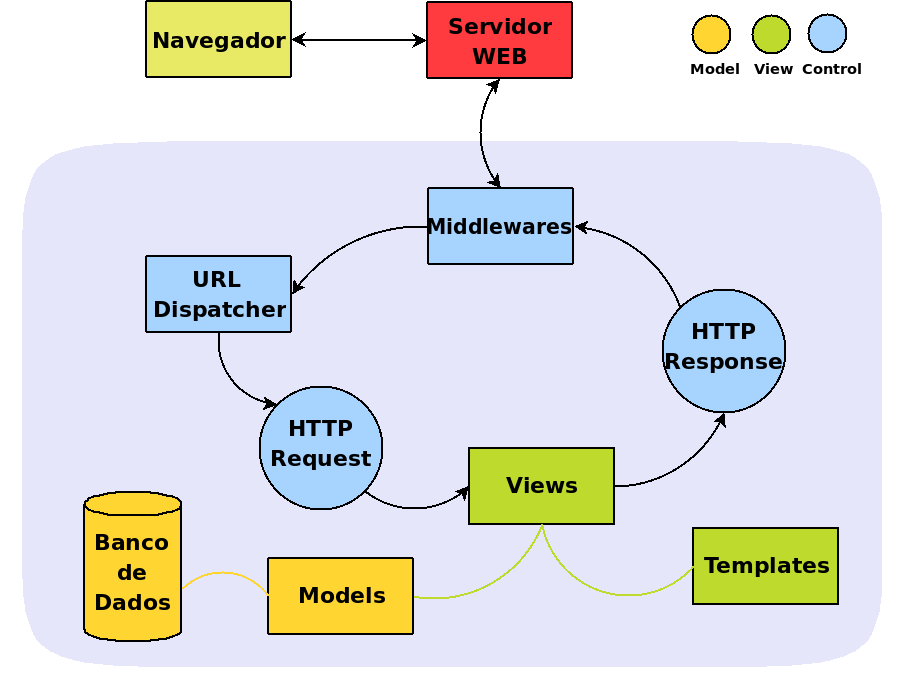
\includegraphics[width=0.7\linewidth]{arquivos/django_arquitetura.png}
        \end{center}
        \caption{Arquitetura MTV do Django}
        \label{django_arquitetura}
    \end{figure}

    No caso da arquitetura MTV, o \textit{framework} Django é o que faz as vezes de controlador da arquitetura MVC. Sendo assim, na arquitetura MTV, o \textit{Controller} não é responsável pela lógica do negócio e sim pelo funcionamento do sistema. Além de \textit{models}, \textit{views} e \textit{templates}, no Django há também o \textit{URL dispatcher},\textit{middlewares} e \textit{handlers} e são estes que são encarados como \textit{Controller}.

    O \textit{URL dispatcher} é o componente responsável em analisar os endereços requisitados pelo cliente e redirecionar essa requisição para a aplicação correta. Já o \textit{middleware} é um conjunto de componentes que realizam pré e pós filtragens nas requisições, o que possibilita funcionalidade como internacionalização de uma aplicação e gerenciamento de sessões autenticadas.

    No \textit{Model}, são escritas as classes que designarão as tabelas no banco de dados. A manipulação dessas tabelas ocorre através do ORM (mapeamento objeto relacional) e, por isso, não é necessária a escrita de \textit{querys} em SQL para a persistência dos dados. Uma outra vantagem é baixa preocupação com qual sistema gerenciador de banco de dados será usado, uma vez que o ORM suporta vários sistemas. Há suporte atualmente para MySQL, PostgreSQL e SQLite.

    Nessa camada também devem ser escritas as regras de acesso às informações, regras para os eventos de cada modelo (métodos \texttt{save}, \texttt{delete}, etc.), e também regras genéricas para eventos que podem ser usados em mais de um modelo (sinais). Toda a lógica de manipulação da informação de uma aplicação estará em seu modelo.

    Na camada \textit{View}, são escritas as regras de negócio e as regras de apresentação do sistema.

    Na camada \textit{Template} é definida a forma de apresentação dos dados que a \textit{View} envia. Com o sistema de \textit{templates} do Django é possível criar heranças, ou seja, um template base contendo a estrutura básica do sistema e templates específicos que herdam as características deste template base e atribuem/criam suas próprias características.

    Com o uso do \textit{framework} Django, um projeto é um conjunto de aplicações. Uma aplicação é uma determinada funcionalidade que compõe um projeto. Por causa disso, há a idéia de aplicações plugáveis no Django que é uma aplicação que pode ser usada em mais de um projeto com nenhuma ou quase nenhuma alteração de código. Isso quer dizer que a aplicação deve ter seus próprios modelos, suas próprias \textit{views}, seus próprios \textit{templates} e encapsular o máximo possível de código que não se enquadre em um desses elementos.
